\documentclass{article}
\usepackage[utf8]{inputenc}

\title{Astronomy 121 Lab 3: Radio Interferometry at X Band}
\author{Vikram Iyer}
\date{\today}

\usepackage{natbib}
\usepackage{graphicx}
\usepackage{listings}
\usepackage[margin=1.0in]{geometry}


\begin{document}

\maketitle

%=======================================================================================

\begin{abstract}
\end{abstract}

%=======================================================================================
%Need
% sun and moon diameter
% least squares plot for each
% 1 hour sun plot
% horizon to horizon sun, filtered
% moon plot, spectrum, filtered
% point source plot, spectrum, filtered
% expected fringe frequencies eq11

   %% rotation matrices
   %11GHz, small sources
   %all info is in f, amp, phase of fringe
   %Baseline = 10m
   %fringe spacing \frac{\lambda}{B}
   %multiplying => 2E_1E_2

   %need precessed ra and dec

   %use UTC to find sidereal time at Long 0deg (HMS), RA tells what part of sky is
   %overhead

   %Use your long oto calcultae offset and find LST

   %RA-LST = HA (hour angle)
   %use lat and

   %state rotation matrices, explain procedure

   %Fringe F depends on  cos(\delta)

   %Formula in lab document is for east west baseline (approx correct for this
   %interferometer)

   %Fringe amplitude vs

   %interf output = cycles/hr

   %Finding frequency
   %Make a guess at value of $\frac{B_y}{\lambda}\cos \delta$
   %Pick a value for RA to get h from LST
   %Least squares with amplitude
   %Save R^2, continue for different guesses, find min
   %with A and B of min, calculate cable length \tau_c

   %total delay
   %$$\Tau_{tot}=\Tau_{g}(h_s)+\Tau_c$$
   %$\Tau_g$ is the geometric path delay between the two telescopes and is a
   %function of time, the hour angle of the source $h_s$
   %$\Tau_c$ is the delay in the cable which will be determined using least-squares.


\section{Introduction}
Interferometry is a common tool in radio astronomy both for the purpose of
correlating multiple signals to improve the signal to noise ratio (SNR)
of weak astronomical signals, as well as to improve the resolution with which
one can observe the sky. The purpose of this lab experiment was to learn and
apply the basic principles of interferometry to measure the diameter of the sun
and the moon, as well as the baseline length of the interferometer from the
known declination of a point source. After recording and processing the raw data
we applied least squares to obtain a function of best fit to the processed data in order to determine the quantities of interest such as source diameter and
baseline.
%=======================================================================================
%citep
\section{Methods}
  \subsection{Interferometer}
  We began this lab experiment by learning about the basics of interferometry as
  well as the details of the system we used for collecting data.

  \subsubsection{A Two Element Interferometer}
  A two-element interferometer consists of two telescopes separated by some
  baseline vector $\vec{b}$. Both telescopes receive radiation from the observed
  source and these signals are multiplied together to form the output. Because
  of the separation of the two telescopes, there is a delay between the time at
  which waves from the source reach the first telescope and the second one.

  We can define the signals that each antenna detects as follows:
  \[E_{i}(t) = e_{1}(t) + e_{2}(t)\]
  \[E_{j}(t) = e_{1}(t-\tau_{1}) + e_{2}(t-\tau_{2})\]

  Correlating these received signals from the two antennas results in the
  average power received. The output of correlation should result in a set of
  values in the power spectrum which are significantly larger than the noise.

  \subsubsection{Wurster Hall Interferometer}
  The interferometer consists of two 1m diameter dishes along an approximately
  10m East-West baseline located on the lower roof of Wurster Hall at UC
  Berkeley. Each antenna output is connected to a series of analog
  filters and amplifiers prior to sampling.  After initial amplification and
  filtering at the source of the signal, the inputs are down converted from an
  original frequency of 10.7 GHz. This output is down converted again and
  filtered to a bandwidth of 30MHz. The outputs of the two dishes are then mixed
  and sampled.  The data is collected by an HP digital voltmeter connected via
  GPIB to a Linux workstation. This computer is capable of both recording the
  output as well as controlling the motors to point the telescope. The full
  signal path is shown in \ref{fig:signal_path}.

    \begin{figure}[h!]
    \centering
    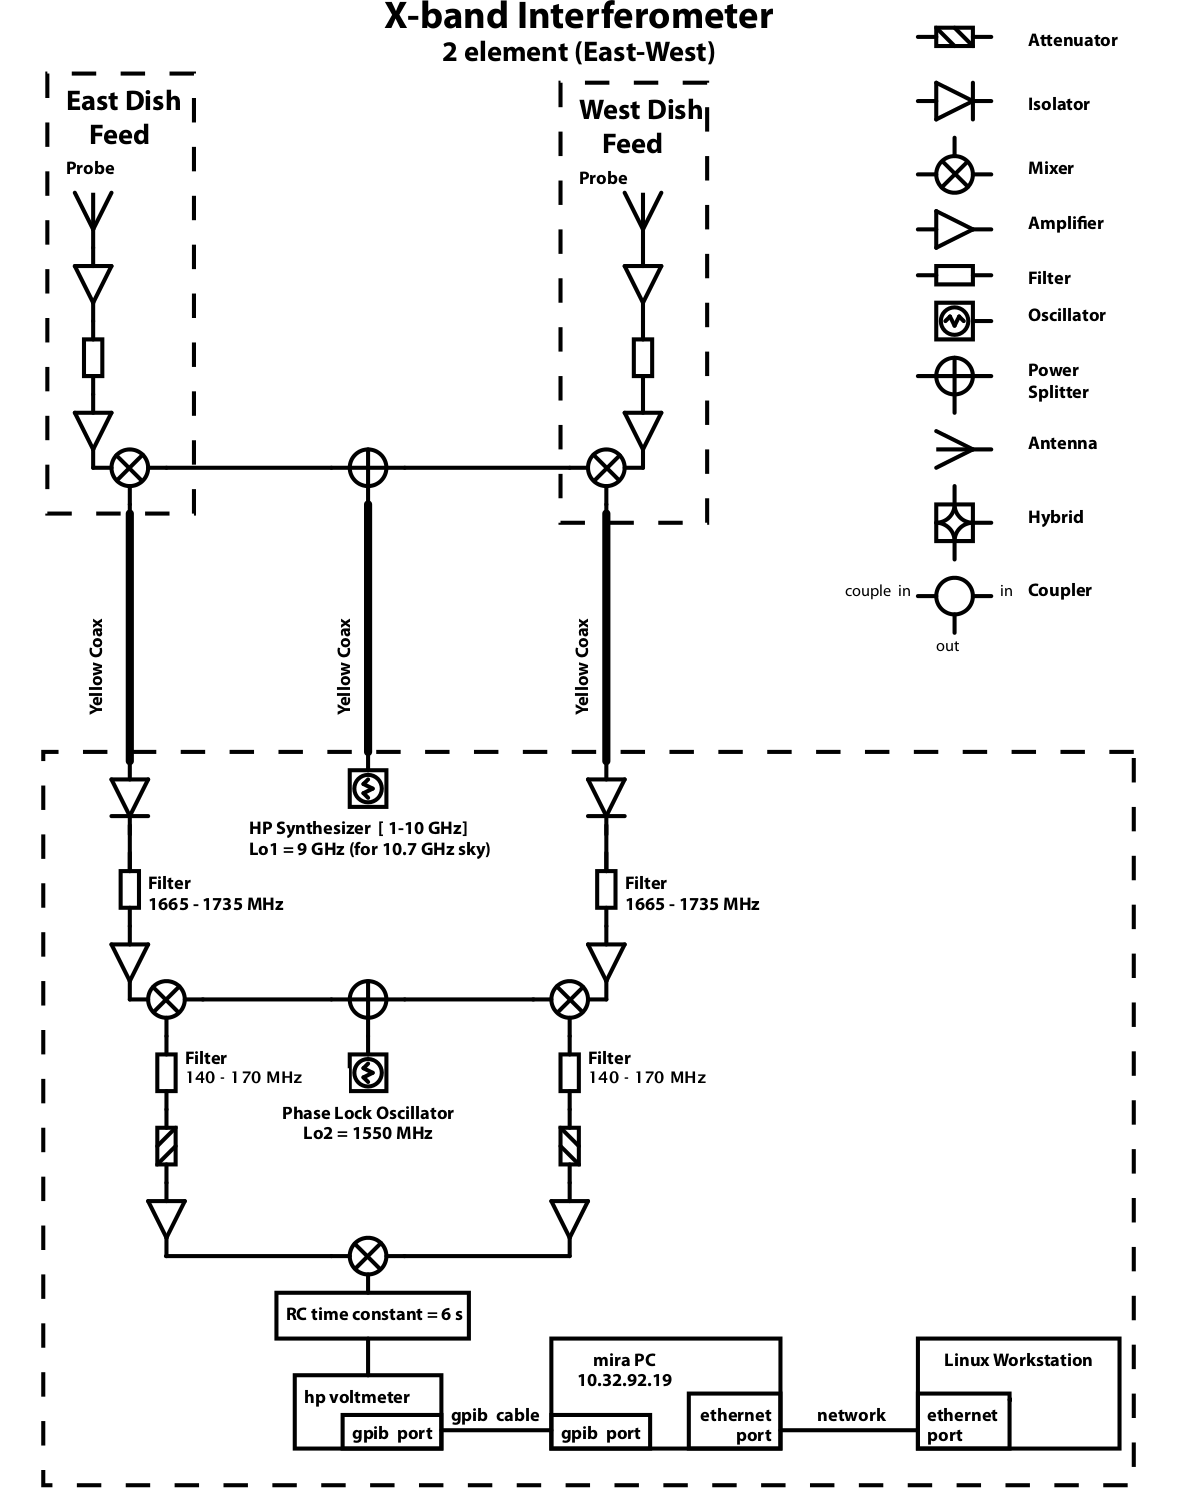
\includegraphics[scale=0.3]{img/signal_path.png}
    \caption{Time domain effects of changing the ratio between the input frequency and the sampling frequency.}
    \label{fig:signal_path}
    \end{figure}

  This interferometer is mechanically limited to an altitude range of
  $15^{\circ}$ to $87^{\circ}$. Additionally, tall buildings such as the
  Campanile and the other half of Wurster Hall further limit the
  interferometer's field of view. The interferometer can be pointed to a
  specified altitude and azimuth value within the range described, and can be
  updated less than every 30 seconds. The dishes' encoders do however
  accumulate error over time and must be reset to a home position every 2-3
  hours.

  \subsection{Coordinate Transformations}
  In order to accurately point the interferometer at sources, we had to
  calculate the positions of sources and update them in real time. The point
  sources of interest all had known known right ascension (RA) and declination
  (DEC) values, however we had to convert these to an altitude and azimuth in
  order to point the telescope.

  To perform the conversion we first converted the given coordinates from
  (RA, DEC) to (HA, DEC) by taking the dot product of the original coordinates
  as a vector with the following rotation matrices.

   \[ {R}_{(\alpha , \delta ) \rightarrow (ha, \delta )} =
      {R}_{(\alpha , \delta) \rightarrow (ha, \delta ),2} \cdot
      {R}_{(\alpha , \delta ) \rightarrow (ha, \delta ),1} \]

   \[ {R}_{(\alpha , \delta ) \rightarrow (ha, \delta ),1} = \\
       \left [ \begin{array}{ccc}
           \cos(LST) & \sin(LST) & 0 \\
           -\sin(LST) & \cos(LST) & 0 \\
           0 & 0 & 1 \\
       \end{array} \right ]  \]

   \[ {R}_{(\alpha , \delta ) \rightarrow (ha, \delta ),2} = \\
       \left [ \begin{array}{ccc}
           1 & 0 & 0 \\
           0 & -1 & 0 \\
           0 & 0 & 1 \\
       \end{array} \right ]  \]

  After converting the values to terms of HA, which is dependent on a
  terrestrial position, we converted from (HA, DEC) to (ALT, AZ) based on our
  latitude $\phi$ using the following matrix.
   \[ {R}_{(ha , \delta ) \rightarrow (az, alt)} = \\
       \left [ \begin{array}{ccc}
           -\sin(\phi) & 0 & \cos(\phi) \\
           0 & -1 & 0 \\
           \cos(\phi) & 0 & \sin(\phi) \\
       \end{array} \right ]  \]

  In order to accurately determine RA and DEC at the time of observation, we
  precessed the catalog values of RA and DEC for the epoch 2000. To perform this
  calculation we used the Python module PyEphem. In addition PyEphem
  contains useful options to calculate the altitude and azimuth of the sun and
  moon. This is particularly useful for the moon as it accounts for the effects
  of observing an object so close to the Earth. We also used the
  \lstinline{ephem.FixedBody} object to actually perform the calculation of
  the altitude and azimuth for the point sources when collecting data. The
  details of the implementation can be found in \lstinline{observe.py}.

  \subsection{Data Collection}
  As explained previously, the interferometer is connected to a Linux computer
  that is remotely accessible. In order to collect data, we had to ensure that
  the position of the interferometer was updated regularly to be directed at the
  source. Additionally we had to regularly reset the telescope to a reference
  position in order to prevent excessive accumulation of error from the
  encoders. We recalculated the position of the Sun and the Moon every 30
  seconds as their position changed more quickly over time, and every 60 seconds for
  the point sources.

  \subsubsection{Data Collection Script}
  In order to automate our data collection, we wrote a Python script to
  calculate the position of the observed source at a given frequency as well as
  collect and save the data from the digital voltmeter (DVM). The script itself is
  divided into two main functions that run in separate threads; the first of
  these functions \lstinline{controller} calculates the position of the source
  every \lstinline{t} seconds and re-points the telescope while the
  \lstinline{recordData} function records data from the DVM and saves the output
  to a specified file. The source position updates were calculated based on
  updating the time of the \lstinline{ephem.Observer} object used by PyEphem to
  compute the altitude and azimuth. As shown above, while our location on Earth
  was fixed, converting (RA,DEC) to (ALT, AZ) at a specific location requires
  the local sidereal time (LST) which we obtained using the
  \lstinline{ephem.now} function.

  Both the data record data and controller were run in separate threads so that
  we could record data continuously rather than having to pause and resume data
  collection to re-point the telescope every 30 seconds. In addition both
  threads were run as daemons to ensure consistency in the data (ie to account
  for cases in which the pointing may have failed, at which point recording data
  additional data would have been misleading). All functions used Python's
  logging utility to record detailed debug and warning messages for reference
  during data analysis. The full data collection script is available with
  detailed function documentation in \lstinline{observe.py}.

  \subsubsection{Observed Sources}
  We observed a variety of sources including the Sun from horizon to horizon, as
  well as the Moon and point sources such as 3C144 (the Crab Nebula). We began
  by observing the Sun for a period of 1 hour, mainly to ensure that our data
  collection script was properly tracking and recording sources. After this we
  observed the Sun from horizon to horizon to gather data necessary for
  determining its diameter. We attempted to observe the moon multiple times,
  however most of these observations were within a few days of a new moon at
  which point only 15\% of the moon was actually illuminated. We obtained
  an additional observation of the moon for 4 hours approximately a week after
  the new moon at which point 30\% was illuminated. We attempted to observe
  multiple point sources including Orion, the Crab Nebula, and M17 as well.

  \subsection{Data Processing}

%=======================================================================================

\section{Results \& Discussion}

%=======================================================================================

\section{Conclusion}

Code and results are available online at: https://github.com/viyer/astro121

%   \bibliographystyle{plain}
%   \bibliography{references}
\end{document}
